\newlparagraph{Definition}


\newlparagraph{Stacks}

\newlparagraph{Geometry}
The idea behind choosing a type of meta surface was: To use a simple and easy to manufacture geometry and achieve complex transmission spectra by stacking these simple layers on top of each other. It is essential to use particles of at least $C^4$ rotational symmetry to enable the layer to affect x and y polarizations differently. A fitting geometry are rectangular meta surface particles.

\begin{figure}[H]
\centering
\begin{subfigure}{.5\textwidth}
    \centering
    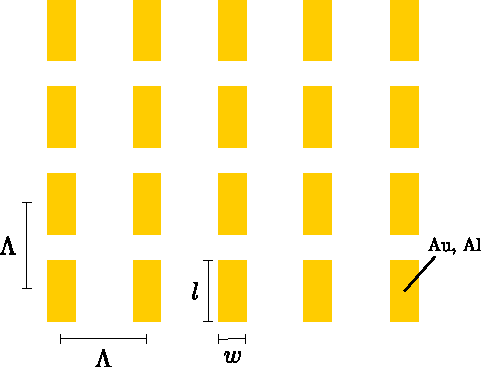
\includegraphics[width=.9\linewidth]{bg_MS}
    \caption{rectangles}
    \label{}
\end{subfigure}%
\begin{subfigure}{.5\textwidth}
    \centering
    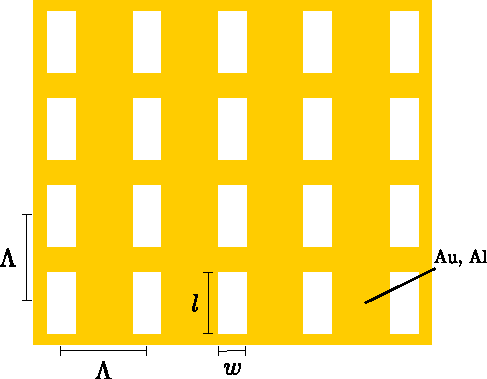
\includegraphics[width=.9\linewidth]{bg_MS_holes}
    \caption{rectangular holes}
    \label{}
\end{subfigure}
\caption{The rectangular particles of width $w$ and length $l$ are arranged on a square matrix with Periode $\Lambda$ in x and y direction. They are made of Gold or Aluminium. The second geometry (b) is inverse to the first in that wherever there was material now light can transmit freely. Both layers also have thickness $t$.}
\label{fig:bg:MS}
\end{figure}
